% TikZ redraw for exercise 3-14
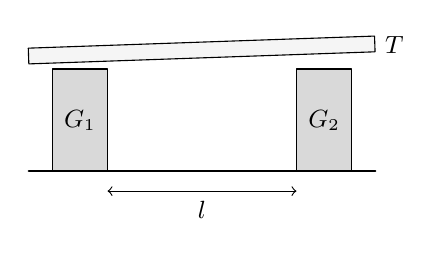
\begin{tikzpicture}[font=\small,line cap=round,line join=round]
\filldraw[fill=gray!30](-.7,0)rectangle(0,1.3);\filldraw[fill=gray!30](2.4,0)rectangle(3.1,1.3);\draw[thick](-1,0)--(3.4,0);\filldraw[fill=gray!8,rotate around={2:(0,1.4)}](-1,1.4)rectangle(3.4,1.6);\node at(-.35,.65){$G_1$};\node at(2.75,.65){$G_2$};\node[right]at(3.4,1.6){$T$};\draw[<->](0,-.25)--node[below]{$l$}(2.4,-.25);
\end{tikzpicture}
